\documentclass{article}

% if you need to pass options to natbib, use, e.g.:
%     \PassOptionsToPackage{numbers, compress}{natbib}
% before loading neurips_2024


% ready for submission
\usepackage{MPL}
\usepackage{graphicx}

% to compile a preprint version, e.g., for submission to arXiv, add add the
% [preprint] option:
%     \usepackage[preprint]{neurips_2024}


% to compile a camera-ready version, add the [final] option, e.g.:
%     \usepackage[final]{neurips_2024}


% to avoid loading the natbib package, add option nonatbib:
%    \usepackage[nonatbib]{neurips_2024}


\usepackage[utf8]{inputenc} % allow utf-8 input
\usepackage[T1]{fontenc}    % use 8-bit T1 fonts
\usepackage{hyperref}       % hyperlinks
\usepackage{url}            % simple URL typesetting
\usepackage{booktabs}       % professional-quality tables
\usepackage{amsfonts}       % blackboard math symbols
\usepackage{nicefrac}       % compact symbols for 1/2, etc.
\usepackage{microtype}      % microtypography
\usepackage{xcolor}         % colors
\usepackage{graphicx}
\usepackage{subcaption}
\usepackage{amsmath}


\title{Temporal Driver Activity Detection}

% The \author macro works with any number of authors. There are two commands
% used to separate the names and addresses of multiple authors: \And and \AND.
%
% Using \And between authors leaves it to LaTeX to determine where to break the
% lines. Using \AND forces a line break at that point. So, if LaTeX puts 3 of 4
% authors names on the first line, and the last on the second line, try using
% \AND instead of \And before the third author name.


\author{%
  Shuvam Aich \\
  Department of Computer Science\\
  University of Stuttgart\\
  Stuttgart, Germany \\
  \texttt{st187673@stud.uni-stuttgart.de} \\
  \And
  Mugdha Asgekar \\
  Department of Computer Science\\
  University of Stuttgart\\
  Stuttgart, Germany \\
  \texttt{st188427@stud.uni-stuttgart.de} \\
  \AND
  Prateek Chaturvedi \\
  Department of Computer Science\\
  University of Stuttgart\\
  Stuttgart, Germany \\
  \texttt{st190139@stud.uni-stuttgart.de} \\
  \And
  Mahdi Jafarkhani \\
  Department of Computer Science\\
  University of Stuttgart\\
  Stuttgart, Germany \\
  \texttt{st186851@stud.uni-stuttgart.de} \\
}

\begin{document}

\maketitle


\begin{abstract}
Driver activity detection in videos presents unique challenges due to the temporal dependencies inherent in video data. This report addresses these challenges by employing a sliding window approach to analyze sequences of frames, which helps to preserve context and improve detection performance. This method uses a fixed-size window that moves across the video, capturing localized segments. Each window is then processed using a pre-trained I3D model to predict the activity. Model performance is evaluated using metrics such as the midpoint hit criteria and Intersection over Union (IoU). The I3D model, a deep learning architecture that extends 2D convolutional neural networks into 3D, is used to capture spatiotemporal features, achieving an average accuracy of 82.26\%. The study also explores advanced model architectures like transformers, temporal CNNs, and recurrent neural networks (RNNs) to further enhance accuracy. Our code and experiment results are available on
the \href{https://github.com/M-Jafarkhani/DriveAndActInferenceDemo}{GitHub}.
\end{abstract}


\section{Introduction}

Activity detection in videos is a challenging problem because videos contain temporal dependencies where activities evolve over time. Unlike static images, where an object classification model can predict a single label per frame, videos require models to understand the progression of actions. A direct classification approach, where each frame is independently classified, often fails to capture contextual information and temporal dependencies, leading to inaccurate predictions. To solve this problem, we employed a sliding window approach, which makes it possible to analyze a sequence of frames together rather than in isolation. The key idea behind the sliding window approach is to use a fixed-size window that moves over the video, capturing a localized segment at each step. This enables better context preservation and helps improve detection performance. A video typically consists of thousands of frames, and activities often span across multiple consecutive frames rather than occurring in a single instance. Using a window of frames allows the model to capture transitions effectively. The sliding window approach retains context from nearby frames, helping the model understand activity progression. Grouping frames into a window allows the model to process fewer but more meaningful segments, which is more efficient.

\section{Dataset Overview}

The Drive\&Act dataset \cite{drive_and_act_2019_iccv} addresses the need for domain-specific action recognition benchmarks, featuring twelve hours of drivers engaged in secondary tasks during both manual and automated driving. Figure \ref{fig:drive-and-act} depicts an overview of the dataset. The dataset includes 9.6 million frames, which is more than four times greater than any other previously published dataset for driver action recognition. The activities are labeled with 83 classes. The dataset is multi-modal, incorporating color, depth, infrared, and 3D body pose data. Six synchronized camera views cover the vehicle cabin to address the issue of limited body visibility. The dataset includes hierarchical activity labels on three levels of abstraction, as well as context annotations.
\subsection{Data Collection}
Data was collected in a static driving simulator to ensure safety, with vehicle surroundings simulated and projected on multiple screens around a converted Audi A3. The simulation software used was SILAB.
Each driver completed twelve different tasks per session, with instructions given on a mounted tablet. Tasks included manual driving, switching to autonomous mode, and responding to unexpected take-over requests. The specific execution of tasks was left to the driver to encourage diverse behavior.
Fifteen participants (4 female, 11 male) with varied body types, driving styles, and familiarity with automation systems were recorded twice, resulting in 30 driving sessions averaging 24 minutes each.
\subsection{Recorded Data Streams}
The dataset includes video data from multiple views and modalities, 3D body and head pose, and features capturing interactions with the car interior. Five near-infrared cameras and a Microsoft Kinect for XBox One were used to capture color, infrared, and depth data. The sensor interfaces were calibrated and synchronized using ROS (Robot Operating System) with global timestamps.
OpenPose was used to determine the 3D upper body skeleton with 13 joints, triangulated from 2D poses from three frontal views (right-top, front-top, left-top). Missing joints were filled using interpolation. OpenFace was also used to obtain the 3D head pose of the driver from all views except the back camera, selecting the most frontal view for each frame. Car-interior features are provided based on 3D primitives, depicting interactions with storage spaces and car controls. Video frames were manually labeled by annotators on three levels of abstraction, resulting in 83 action classes. The annotation scheme includes high-level scenarios, fine-grained activities, and low-level atomic action units.
\subsection{Data Splits}
The dataset is divided into three splits based on the driver's identity, with data from ten subjects for training, two for validation, and three for testing to evaluate generalization to new drivers. Action segments are divided into 3-second chunks for the benchmark, with evaluation scripts provided for comparable results.
The dataset's vocabulary was created based on a literature review of secondary tasks during driving, expert surveys, and analysis of accident reports and naturalistic car studies. The vocabulary covers eight areas: eating and drinking, clothing and accessories, working, entertainment, entering/exiting and car adjustment, body movement, object manipulation, and using vehicle-internal devices. The vocabulary comprises 83 activity labels across three levels of granularity, forming a complexity- and duration-based hierarchy. It also employs three levels of abstraction:
\begin{itemize}
    \item \textbf{Scenarios/Tasks:} The first level consists of twelve tasks that subjects had to complete, which are either typical during manual driving or expected to become common with increasing automation.
    \item \textbf{Fine-grained Activities:} The second level breaks down scenarios into 34 concise categories that retain a clear semantic meaning.
    \item \textbf{Atomic Action Units:} The third level portrays basic driver interactions with the environment, detached from long-term semantic meaning and comprising action, object, and location triplets.
\end{itemize}
\begin{figure}
    \centering
    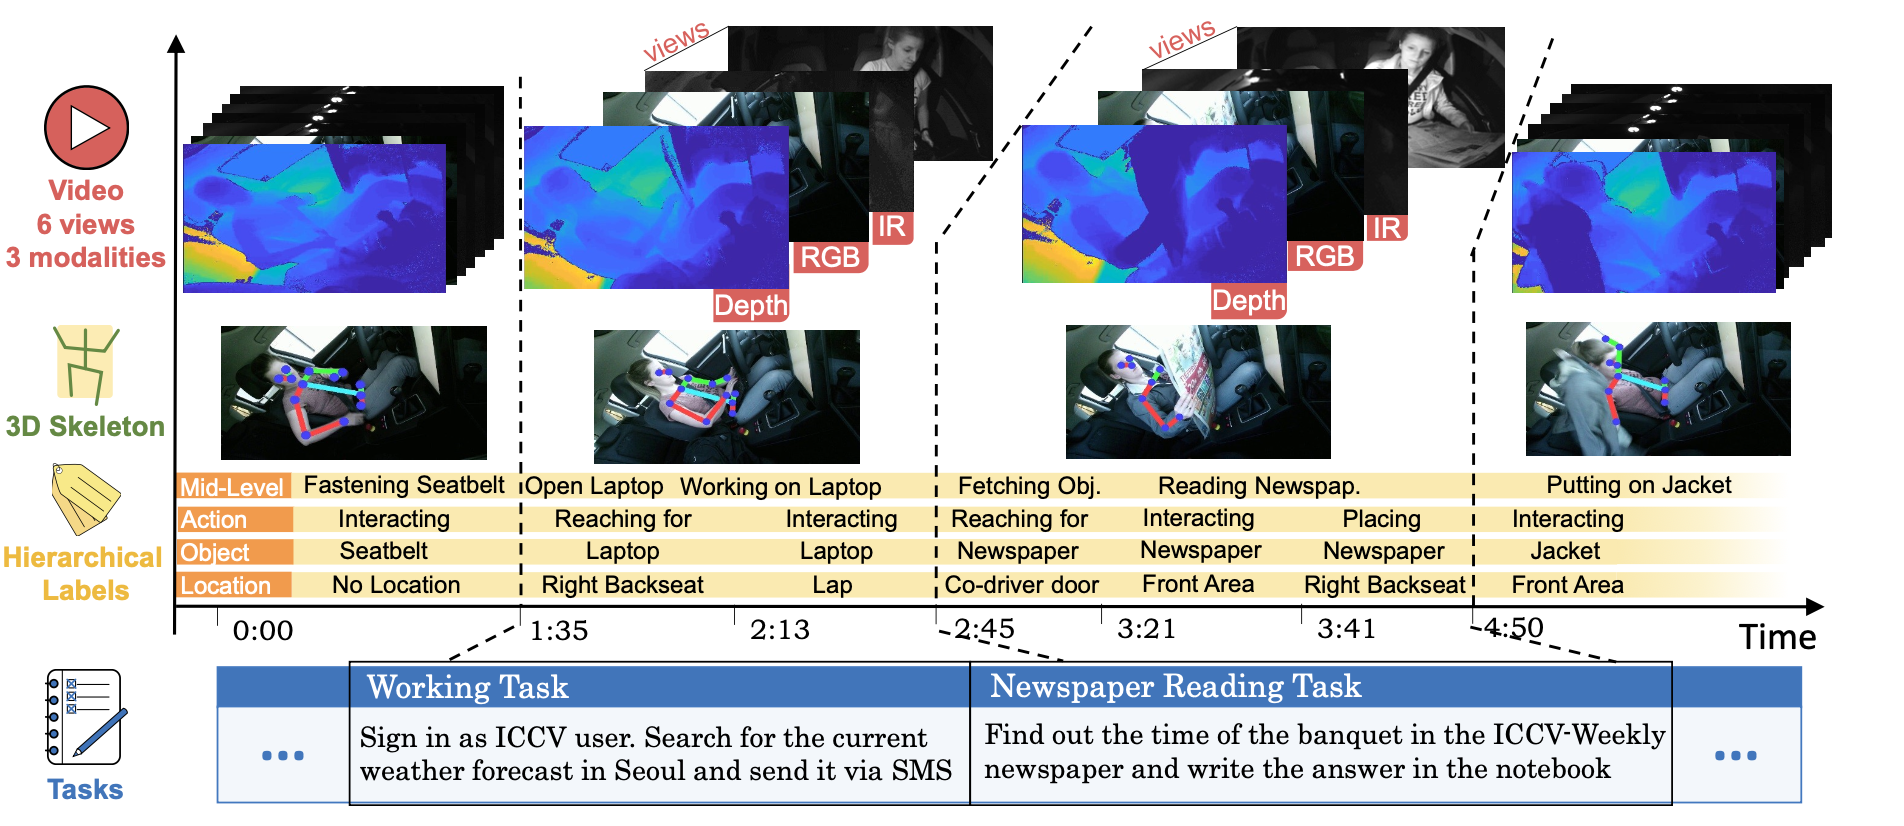
\includegraphics[width=1\linewidth]{figs/drive_and_act.png}
    \caption{Overview of the Drive\&Act dataset for driver behavior recognition. The dataset includes 3D skeletons in addition
to frame-wise hierarchical labels of 9.6 Million frames captured by 6 different views and 3 modalities (RGB, IR and depth). \cite{drive_and_act_2019_iccv}}
    \label{fig:drive-and-act}
\end{figure}
\section{Task 1: Sliding Window}
Activity detection in videos is a challenging problem due to the continuous and dynamic nature of video data. Unlike static images, where an object classification model can predict a single label per frame, videos contain temporal dependencies where activities evolve over time.

A direct classification approach—where each frame is independently classified—often fails to capture contextual information and temporal dependencies, leading to inaccurate predictions. To address this, we employed a sliding window approach, which allows us to analyze a sequence of frames together rather than in isolation.

The key idea behind this approach is that instead of treating the entire video as a single entity or classifying individual frames separately, we use a fixed-size window that moves over the video, capturing a localized segment at each step. This enables better context preservation and helps improve detection performance.

\subsection{Motivation for Using Sliding Window}
A video typically consists of thousands of frames, and activities often span across multiple consecutive frames rather than occurring in a single instance. The sliding window approach is designed to address the following challenges:
\begin{itemize}
    \item \textbf{Temporal Overlap in Activities}: Many activities start and end gradually rather than having sharp boundaries. Using a window of frames allows to capture transitions effectively.
    \item \textbf{Context Awareness}: Classifying each frame in isolation lacks temporal context. The sliding window approach retains context from nearby frames, helping the model understand activity progression.
    \item \textbf{Efficiency and Performance Trade-off}: Instead of analyzing every individual frame separately (which would be computationally expensive), grouping frames into a window allows the model to process fewer but more meaningful segments.
\end{itemize}
\newpage
\subsection{Implementation}
In this section, we describe the implementation details of our sliding window approach for activity detection. The process involves defining a fixed window size and stride to segment the video into overlapping or non-overlapping windows. Each window is then processed using a pre-trained I3D model to generate activity predictions. The following subsections outline these steps in detail.
\subsubsection{Window Size and Stride}
\begin{itemize}
    \item A \textbf{fixed-size window} (e.g. 8, 16, or 32 frames) is defined, which slides across the video.
    \item The \textbf{stride} determines how much the window moves forward after each step.
    \item If the stride is \textbf{small} (e.g., 1 frame), the overlap between windows increases, leading to \textbf{better temporal coverage but higher computational cost}.
    \item If the stride is \textbf{large} (e.g., 8 frames), fewer windows are processed, reducing computation but potentially \textbf{missing fine-grained transitions}.
\end{itemize}

\subsubsection{Processing Each Window}
\begin{itemize}
    \item Each window of frames is sent as input to a pre-trained I3D model.
    \item The model infers on the window and predicts the most likely activity to occur in that segment.
    \item The predicted label is assigned to each frame of the window, along with the confidence scores (Figure \ref{fig:sliding-window-predictions}).
    \item The activity with the highest confidence score is selected for each frame.
    \item As the window progresses, new predictions are generated, leading to a continuous activity timeline.
\end{itemize}

\begin{figure}[ht]
    \centering
    \begin{subfigure}{0.45\textwidth}
        \centering
        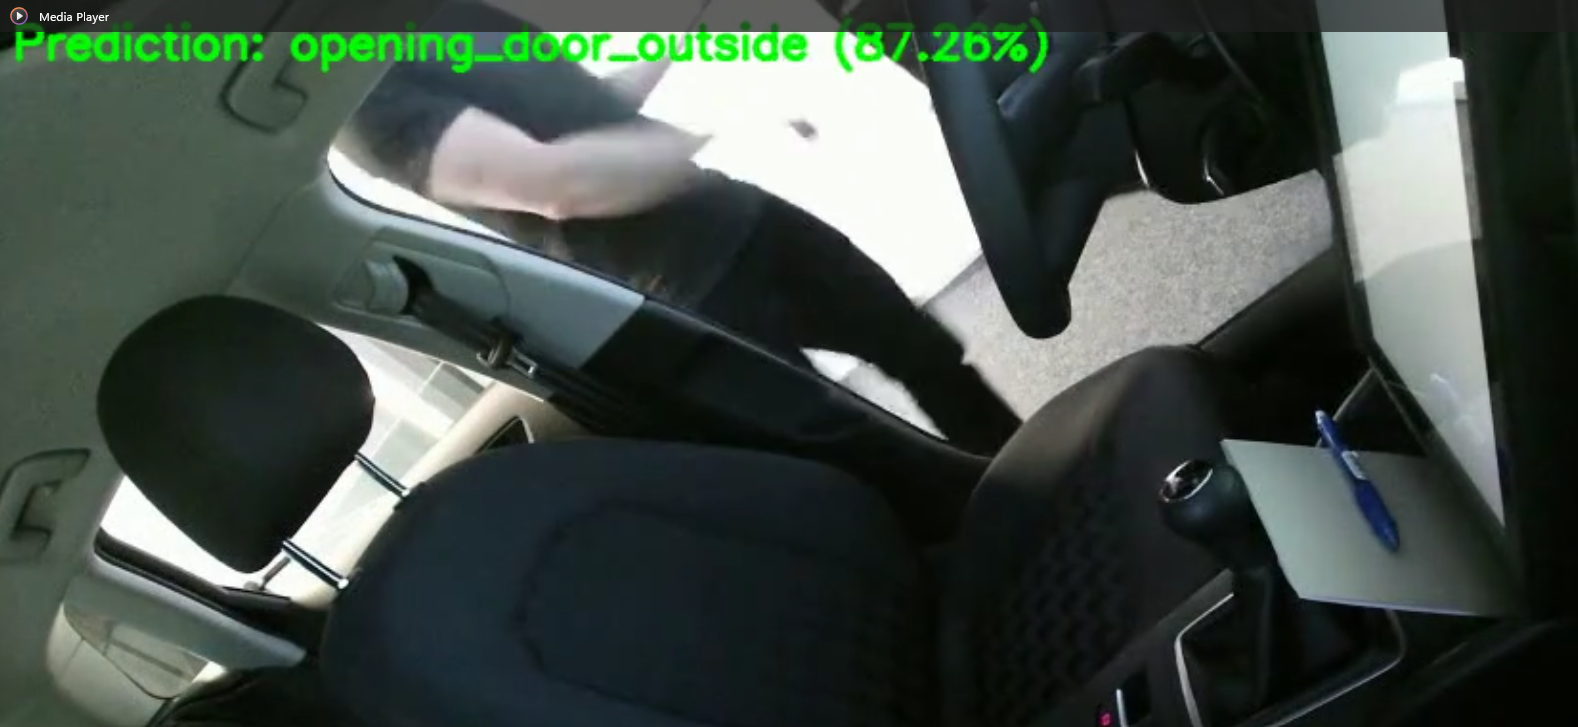
\includegraphics[width=\textwidth]{figs/DAR1.png}
        \caption{Opening door outside}
    \end{subfigure}
    \hspace{0.5cm}
    \begin{subfigure}{0.45\textwidth}
        \centering
        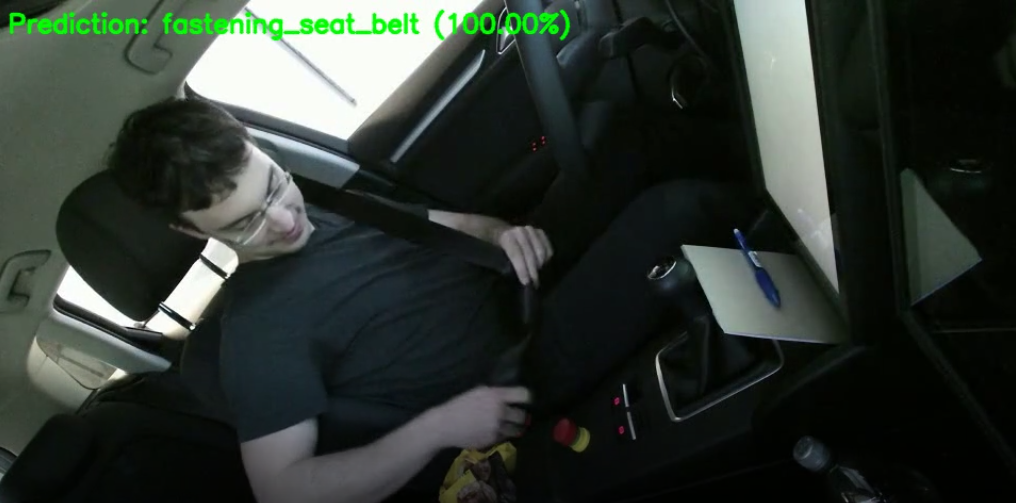
\includegraphics[width=\textwidth]{figs/DAR2.png}
        \caption{Fastening Seat Belt}
    \end{subfigure}

    \vspace{0.5cm}

    \begin{subfigure}{0.45\textwidth}
        \centering
        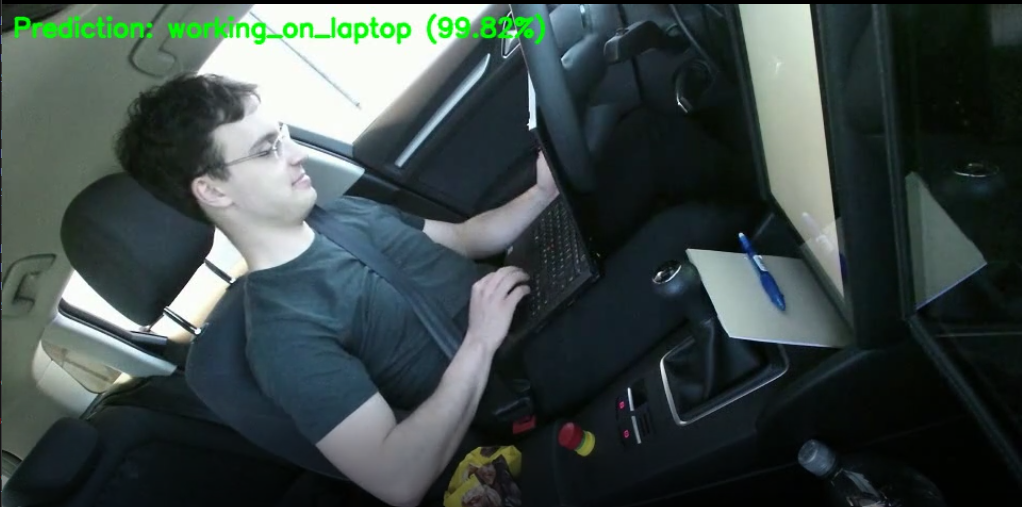
\includegraphics[width=\textwidth]{figs/DAR3.png}
        \caption{Working on Laptop}
    \end{subfigure}
    \hspace{0.5cm}
    \begin{subfigure}{0.45\textwidth}
        \centering
        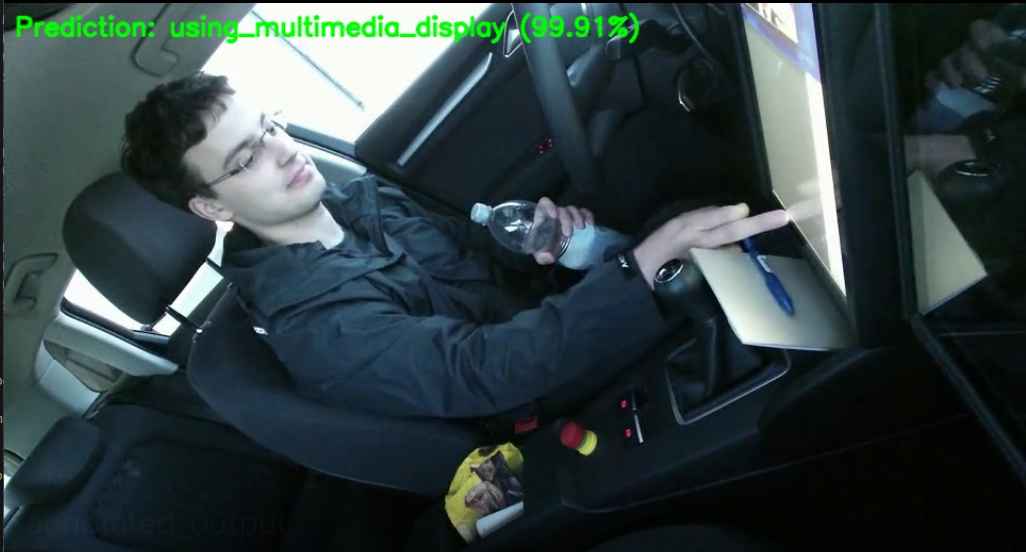
\includegraphics[width=\textwidth]{figs/DAR4.png}
        \caption{Using Multimedia Display}
    \end{subfigure}

    \caption{Grid for multiple predictions using Sliding Window.}
    \label{fig:sliding-window-predictions}
\end{figure}

\section{Metrics}
Evaluating activity detection models requires quantitative metrics that measure how well predictions align with ground truth activities. One of the objectives involved was to develop metrics for the sliding window approach to understand how accurate are the predictions. We employed two key metrics, \textbf{Midpoint Hit Criteria} and \textbf{Intersection over Union (IoU)} as described in detail in the next sections.

\subsection{Midpoint Hit Criteria}

To determine whether a prediction is correct, we used the \textbf{midpoint hit criteria}. For each ground truth activity segment, we computed its midpoint and checked if a predicted segment of the same activity class covered this midpoint. The evaluation steps are as follows:

\begin{itemize}
    \item Compute the \textbf{midpoint} of each ground truth segment as:
    \begin{equation}
        \text{midpoint} = \frac{\text{frame\_start} + \text{frame\_end}}{2}
    \end{equation}
    \item A prediction is counted as a \textbf{true positive (TP)} if it covers the midpoint and belongs to the correct activity class.
    \item If no prediction matches the midpoint, it is considered a \textbf{false negative (FN)}.
    \item Any extra predicted segments that do not match a ground truth midpoint count as \textbf{false positives (FP)}.
    \item Precision and recall for each activity class are calculated as:
    \begin{equation}
        \text{Precision} = \frac{TP}{TP + FP} \times 100
    \end{equation}
    \begin{equation}
        \text{Recall} = \frac{TP}{TP + FN} \times 100
    \end{equation}
    \item Overall precision and recall are computed by aggregating across all activity classes.
\end{itemize}

\subsubsection{Midpoint Hit Analysis: Sliding Window Size vs. Performance}

To evaluate the impact of different sliding window sizes on activity recognition performance, we analyzed precision and recall using the midpoint hit criteria. The figure \ref{fig:sliding-window-predictions} illustrates the mean precision and recall for different test datasets across three sliding window sizes: \textbf{8}, \textbf{16}, and \textbf{32}.


\textbf{Key Observations:}
\begin{itemize}
    \item Larger sliding window sizes (\textbf{32 frames}) generally yield higher precision and recall compared to smaller window sizes (\textbf{8 frames}).
    \item Precision and recall values for a window size of \textbf{16} show intermediate performance, indicating a trade-off between smaller and larger window sizes.
\end{itemize}

Figure \ref{fig:metrics} provides a comparison of how varying window sizes influence detection performance. These results suggest that increasing the sliding window size enhances model robustness, but the optimal selection depends on dataset characteristics and activity granularity.

\begin{figure}[ht]
    \centering
    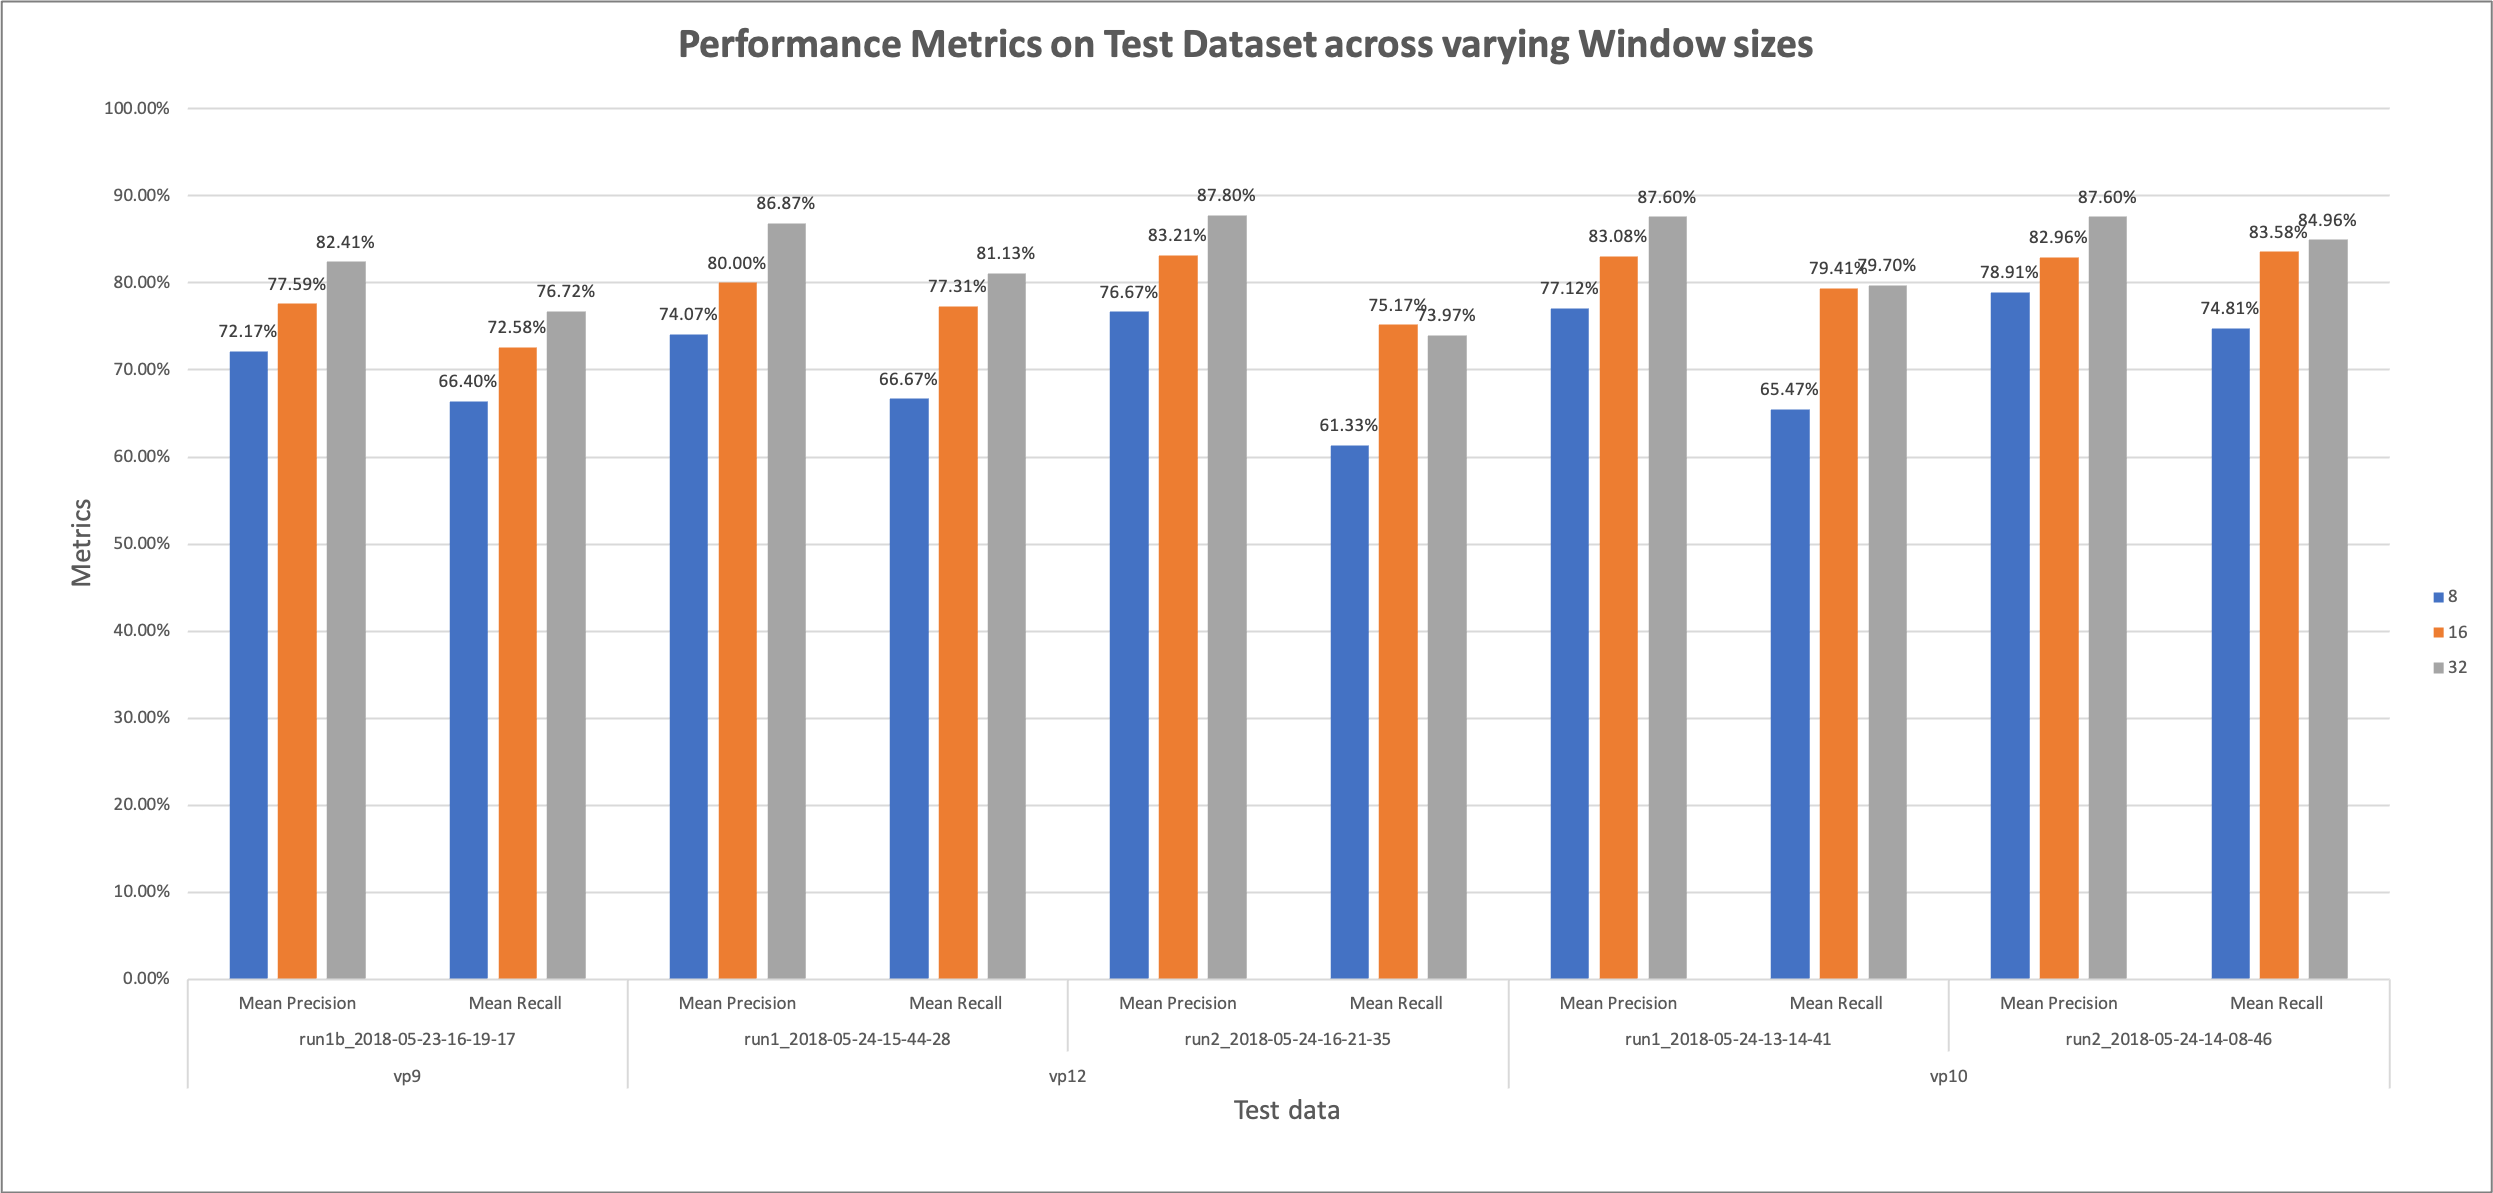
\includegraphics[width=\linewidth]{figs/metrics.png}
    \caption{Performance Metrics on Test Dataset Across Varying Sliding Window Sizes}
    \label{fig:metrics}
\end{figure}

\subsubsection{Midpoint-Based Analysis: Fine-Grained Driver Activity Performance}

In addition to evaluating sliding window effects, we also analyzed the performance of fine-grained driver activity recognition using the midpoint hit criteria. For this analysis, a sliding window size of 16 was used and evaluated on a test dataset.
This evaluation measures prediction accuracy based on how well the model identifies activity occurrences, quantified through precision and recall.

The results, as shown in Figure~\ref{fig:driver-activities}, highlights variations in performance across different activity classes.

\begin{figure}[ht]
    \centering
    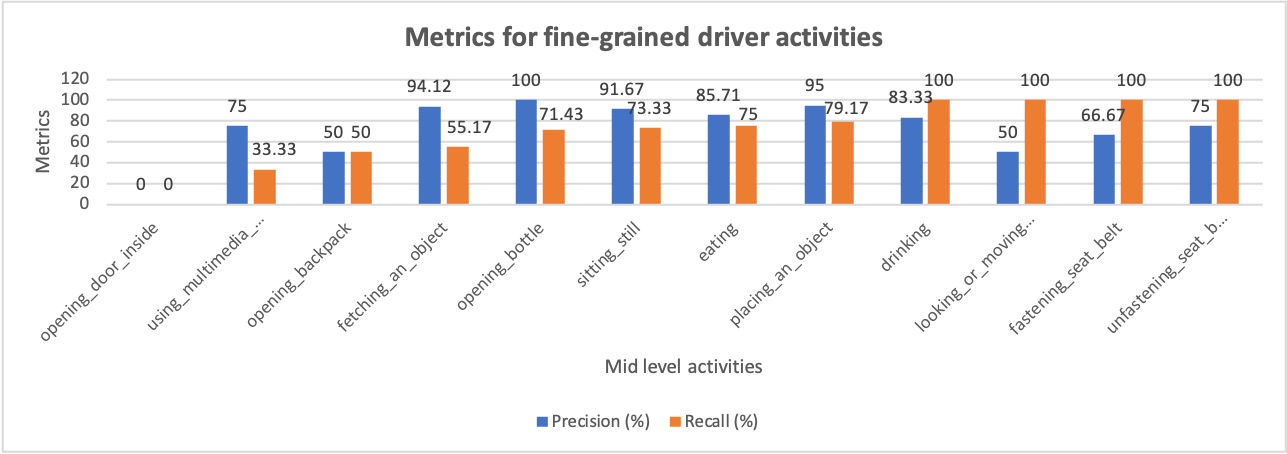
\includegraphics[width=\linewidth]{figs/metrics2.png}
    \caption{Precision and Recall for Fine-Grained Driver Activities}
    \label{fig:driver-activities}
\end{figure}

\textbf{Key Observations:}
\begin{itemize}
    \item Activities such as \textbf{opening a bottle, drinking, and unfastening the seat belt} show high precision and recall, indicating strong prediction accuracy.
    \item Some activities, like \textbf{opening a backpack and fetching an object}, have lower recall values, suggesting that they are harder to detect consistently.
    \item \textbf{Using multimedia controls} was the most challenging action, with both precision and recall at low levels, indicating potential misclassification or lack of training data for this category.
\end{itemize}

By applying the midpoint hit criteria, we ensure a structured evaluation of the model's recognition capability, highlighting both well-detected and challenging activity classes.

\subsection{Intersection over Union (IoU)}

To measure how well the predicted activity windows overlap with the ground truth, we used \textbf{IoU}:

\begin{itemize}
    \item \textbf{Intersection}: The overlapping frames between the ground truth and predicted segment.
    \item \textbf{Union}: The total number of frames covered by both segments.
    \item The \textbf{IoU score} for each ground truth segment is calculated as:
    \begin{equation}
        \text{IoU} = \frac{\text{Intersection}}{\text{Union}}
    \end{equation}
    \item The \textbf{mean IoU} is obtained by averaging the IoU scores across all ground truth segments.
\end{itemize}

Figure \ref{fig:iou-performance} illustrates the mean IoU across different test datasets for three sliding window sizes: 8, 16, and 32.

\begin{figure}[ht]
    \centering
    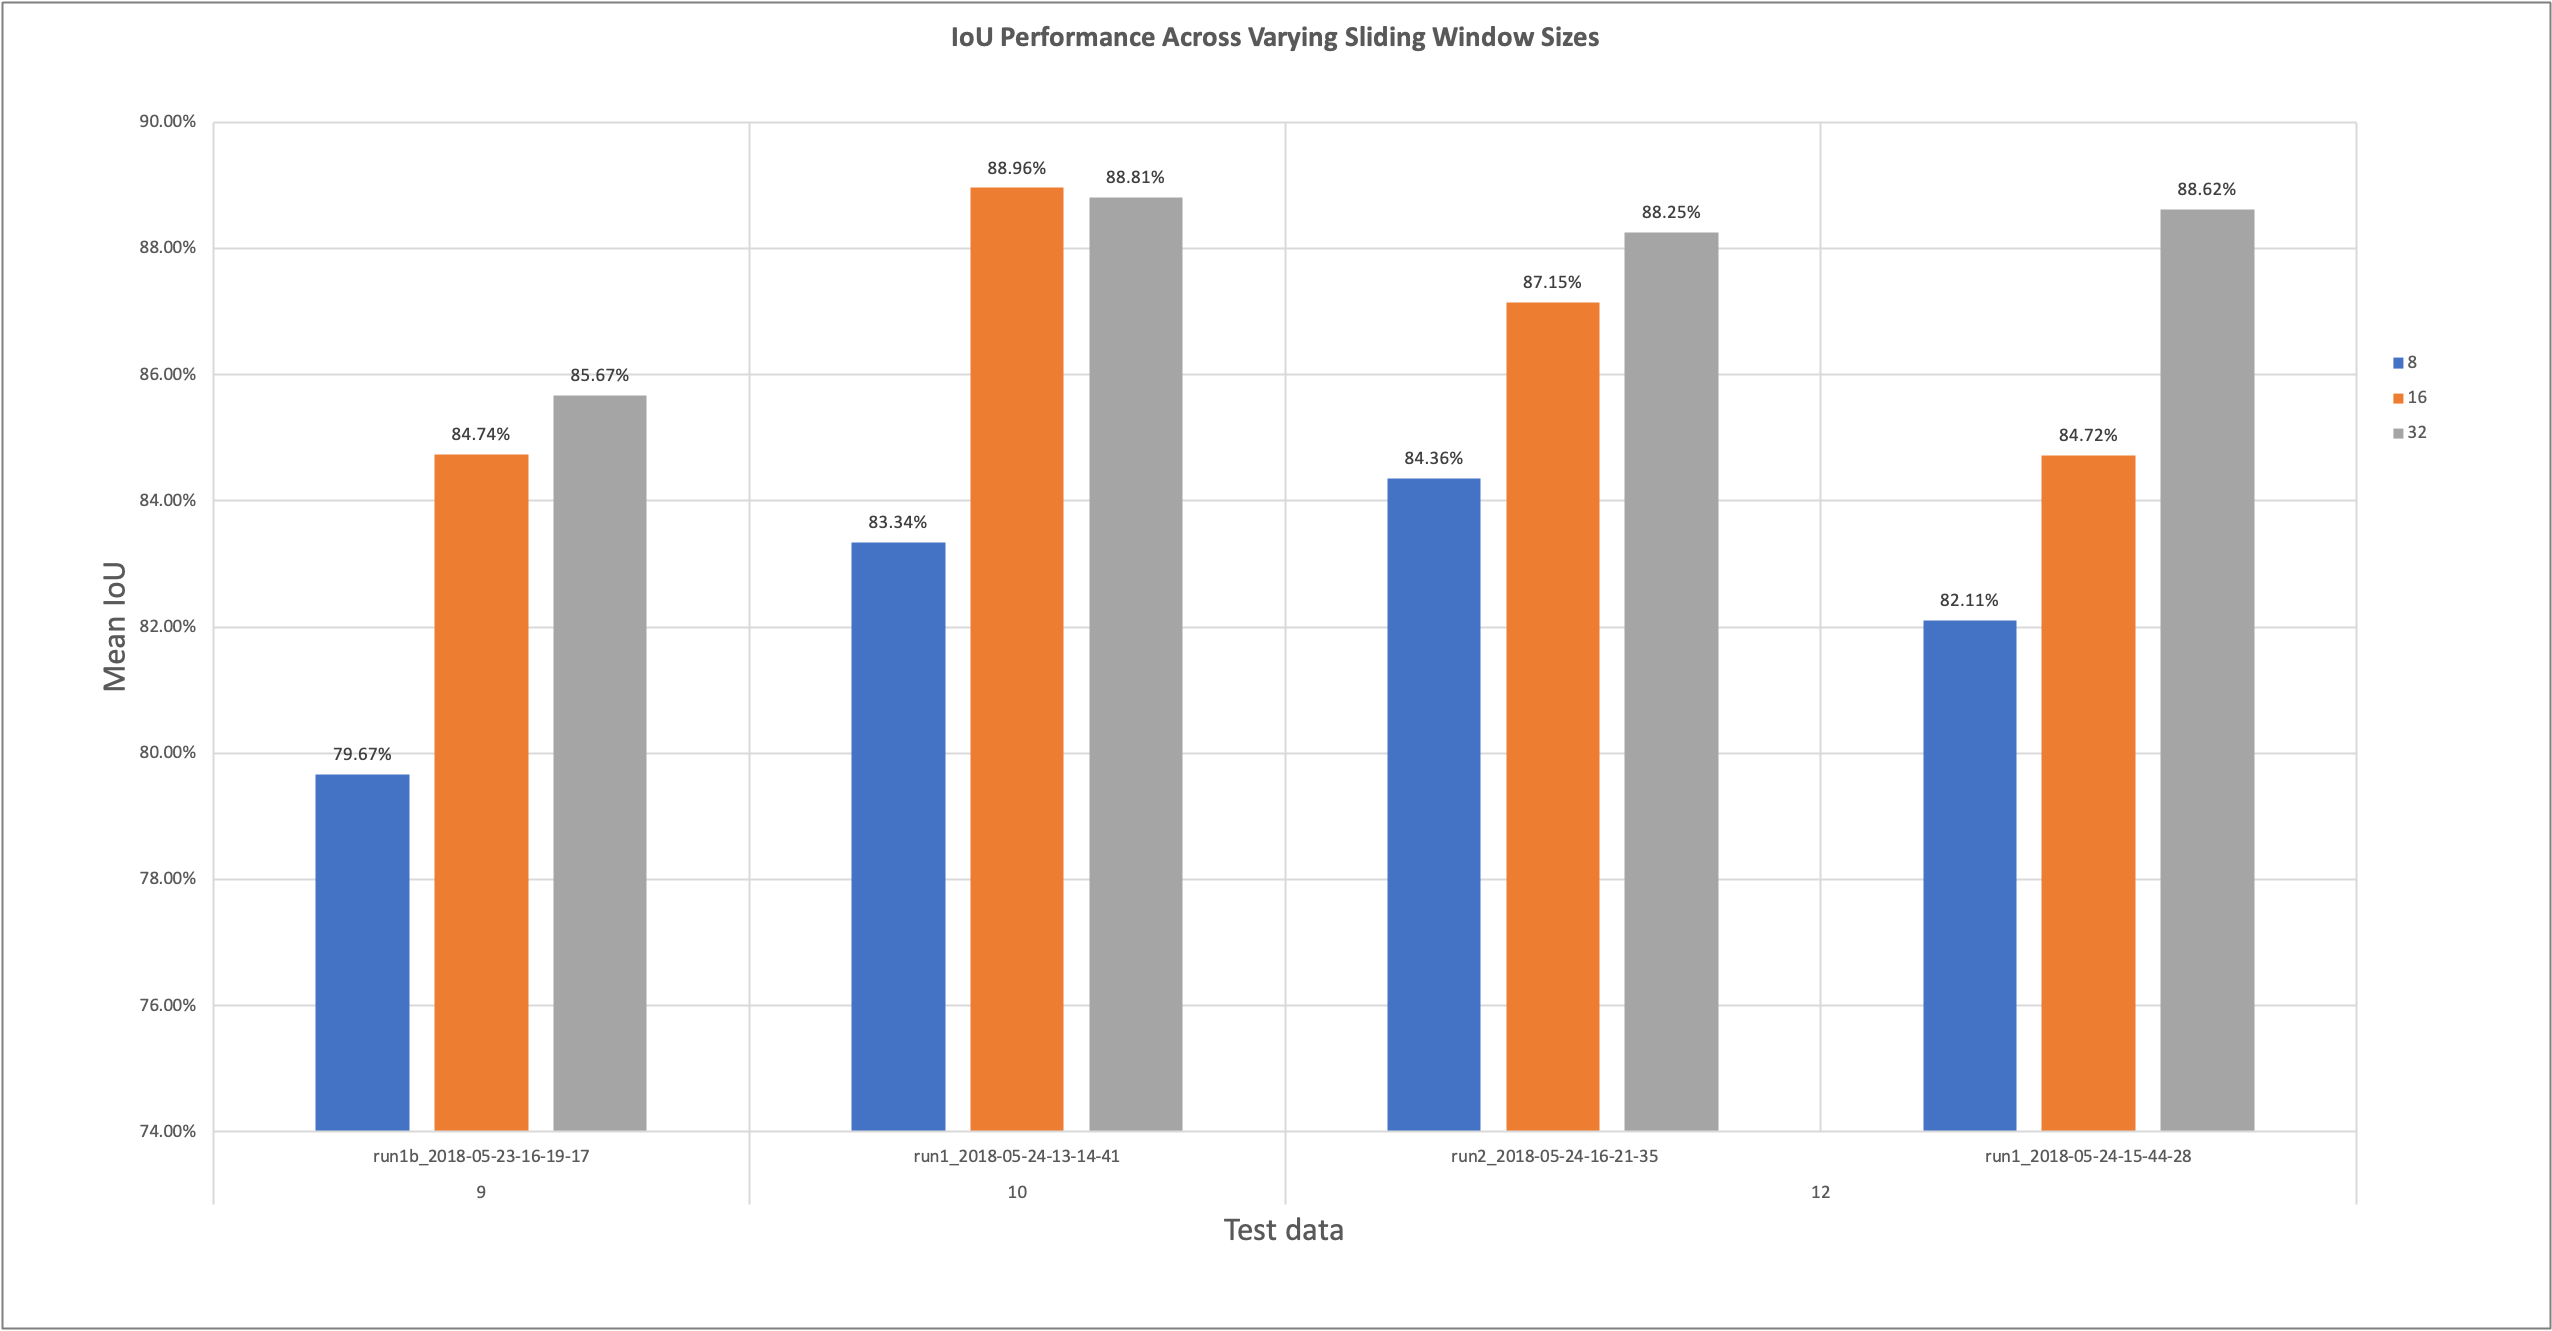
\includegraphics[width=1\linewidth]{figs/iou.png}
    \caption{IoU Performance Across Varying Sliding Window Sizes}
    \label{fig:iou-performance}
\end{figure}

\textbf{Key Observations:}
\begin{itemize}
    \item Larger sliding window sizes (32 frames) generally achieve higher IoU scores, indicating better alignment between predictions and ground truth.
    \item Smaller window sizes (8 frames) tend to have lower IoU scores, possibly due to fragmented segment predictions.
    \item The trend is consistent across multiple test datasets, reinforcing the positive impact of larger window sizes on IoU performance.
\end{itemize}

These results demonstrate that choosing an optimal sliding window size significantly affects overlap accuracy, with larger windows generally providing better segmentation alignment.

\subsection{Final Evaluation Results}
We analyzed different sliding window sizes on activity detection performance, using metrics like precision, recall and IoU, supports the idea that larger window sizes generally improve model robustness, though the optimal selection depends on dataset characteristics and activity granularity. The detailed results in Table \ref{tab:sliding_window_results} indicates this trend.
  
\begin{table}[h]
    \renewcommand{\arraystretch}{1.5}
    \centering
    \begin{tabular}{c|c|c|c}
        \hline
        \textbf{Window Size} & \textbf{Overall Precision (\%)} & \textbf{Overall Recall (\%)} & \textbf{IoU (\%)} \\
        \hline
        8  & 75.39  & 66.11 & 82.37 \\
        16 & 81.41  & 77.21 & 86.39\\
        32 & \textbf{87.46}  & \textbf{79.90} & \textbf{87.84}\\
        \hline
    \end{tabular}
    \vspace{10pt}
    \caption{Average Overall Precision, Recall and IoU for Different Sliding Window Sizes}
    \label{tab:sliding_window_results}
\end{table}

\section{Task 2: Neural Detection Model}
Manuel and Roitberg \cite{drive_and_act_2019_iccv} evaluated various models for fine-grained driver activity recognition using the Drive\&Act dataset. They tested different approaches, including CNN-based methods (like C3D, P3D ResNet, and I3D) and body pose-based methods. They found out that the Inflated 3D ConvNet (I3D), an extension of the Inception-v1 network with 3D convolutions, achieved the highest accuracy (69.57\% on Validation, and 63.64\% on test) among all tested models for recognizing fine-grained driver activities.
I3D also outperformed body pose-based methods, which were less effective in classifying actions despite incorporating spatial and temporal streams.
In atomic action unit classification, I3D performed best in recognizing actions (56.07\%) and objects (56.15\%), though body pose-based approaches were better at identifying locations (56.5\%).Although for cross-view action recognition, I3D models struggled with domain shifts, performing significantly worse when tested on unseen views.
\subsection{I3D Model}
The Two-Stream Inflated 3D ConvNet (I3D) \cite{carreira2018quovadisactionrecognition} is a deep learning model designed for video action recognition. It extends 2D convolutional neural networks (CNNs) into 3D by "inflating" their filters and pooling kernels to operate in both spatial and temporal dimensions. This allows the model to effectively capture motion patterns in videos (Figure \ref{fig:i3d}).
\subsubsection{Key Features of I3D}
\begin{itemize}
    \item \textbf{3D Convolutions}: Unlike traditional 2D CNNs that process images independently, I3D uses 3D convolutional layers to extract spatiotemporal features from videos.
    \item \textbf{Inflation from 2D Networks}: The model is based on the Inception-v1 architecture, with its 2D filters expanded into 3D. This allows it to reuse ImageNet pre-trained weights, improving efficiency and performance.
    \item \textbf{Two-Stream Configuration}: I3D processes both RGB frames (spatial information) and Optical flow (motion information). These two streams are trained separately and their outputs are fused at the end.
\end{itemize}

\begin{figure}[ht]
    \centering
    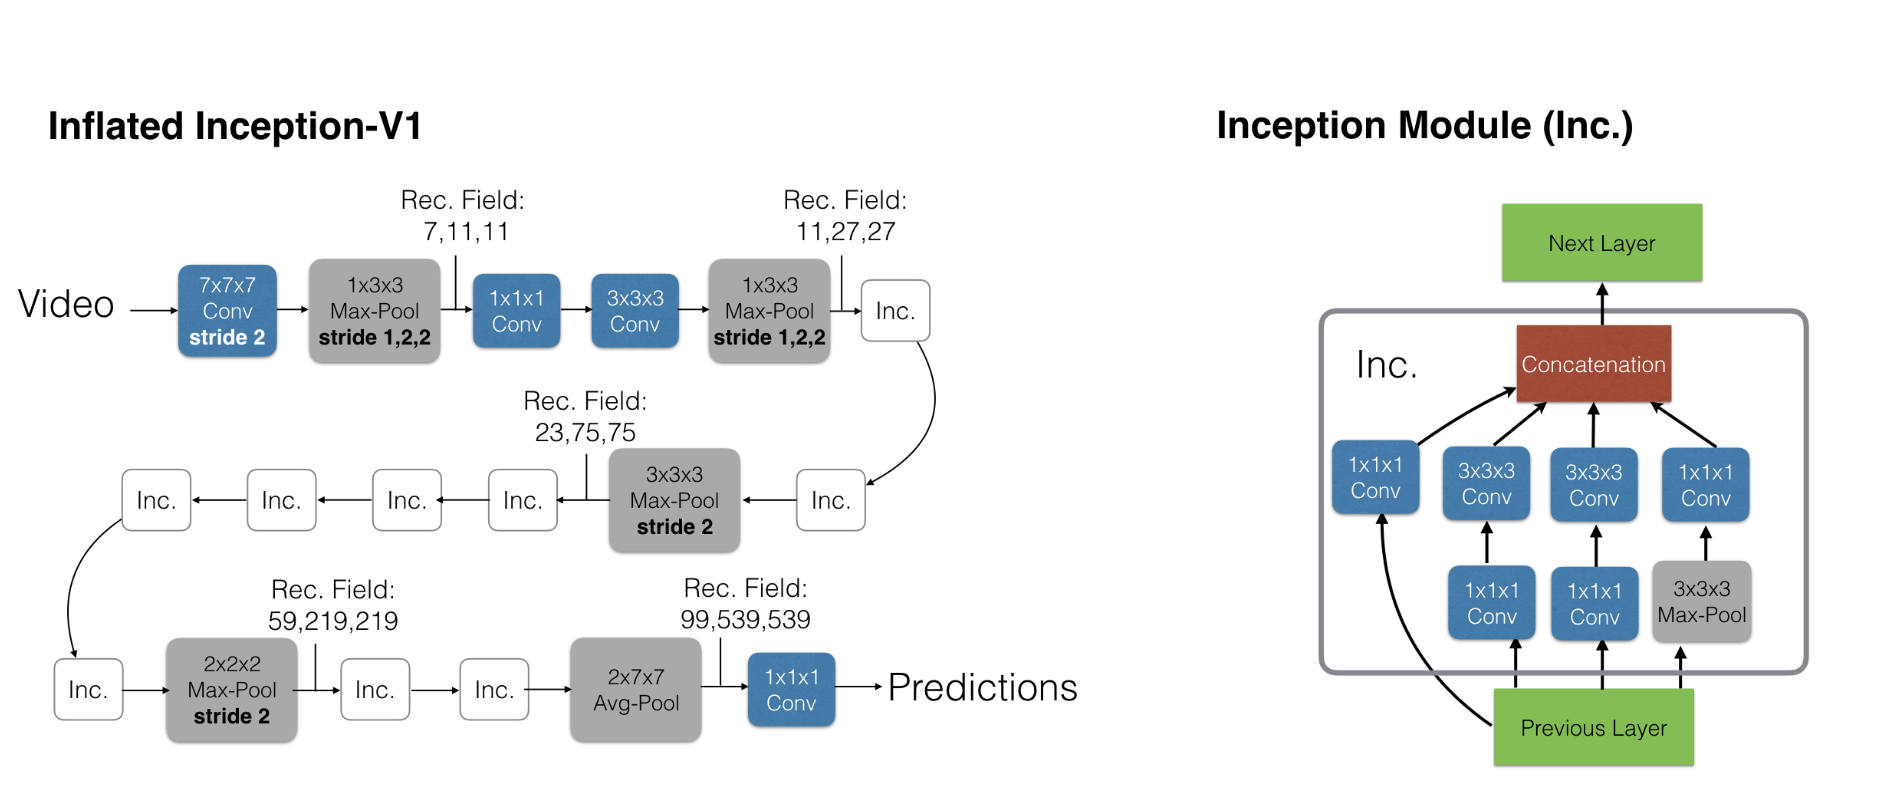
\includegraphics[width=0.9\linewidth]{figs/i3d.png}
    \caption{The Inflated Inception-V1 architecture (left) and its detailed inception submodule (right). The strides of convolution and pooling
operators are 1 where not specified, and batch normalization layers, ReLu’s and the softmax at the end are not shown. The theoretical
sizes of receptive field sizes for a few layers in the network are provided in the format “time,x,y” – the units are frames and pixels. The
predictions are obtained convolutionally in time and averaged.\cite{carreira2018quovadisactionrecognition}}
    \label{fig:i3d}
\end{figure}

\subsection{I3D Model as baseline model}
We utilized the I3D model for recognition in our project. We evaluated a pre-trained I3D model and performed inference on all videos in the Kinetic Color category. Figure \ref{fig:i3d-acc} illustrates the model's accuracy on the Drive\&Act dataset. The dataset includes 15 viewpoints, each comprising two runs, except for viewpoint 9, which lacked annotation for the second run. The average accuracy is 82.26\% for our baseline model.
We noticed the main reason for misclassfying each frame to its action is either by:
\begin{itemize}
    \item \textbf{Latency in Annotation}: Since human-labeled annotations (ground truths) lack a strict consensus on the exact start time of an action, some degree of misclassification is inevitable. In this context, misclassifying an action by at most 10 frames is considered acceptable or, in other words, irreducible.
    \item \textbf{Fast Switching Actions}: The model exhibited rapid transitions between actions, sometimes within less than 3 frames. This behavior was of particular interest to us, and we hypothesized that applying a neural network or transformer architecture on top of the I3D model could help reduce this misclassification.
\end{itemize}
\begin{figure}[ht]
    \centering
    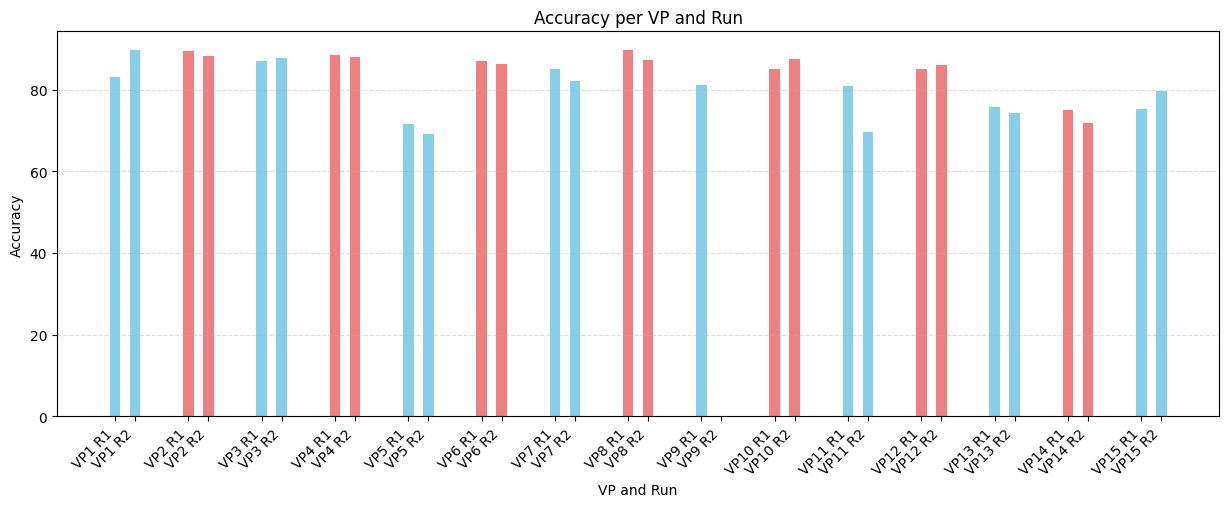
\includegraphics[width=1\linewidth]{figs/i3d-acc.png}
    \caption{Accuracy for recognition task with I3D model on all viewpoints and runs on Kinetic Color category, Drive\&Act dataset}
    \label{fig:i3d-acc}
\end{figure}
\newpage
\subsection{Extending I3D Model}
To further improve the performance of our detection model, we extended the I3D-based approach by exploring alternative architectures and preprocessing techniques. This section details the preprocessing steps taken to prepare the dataset and the enhancements applied to the model, along with the challenges encountered during training and optimization.
\subsubsection{Preprocessing}
The input data utilized in this study was originally trained using the I3D model, which generated class probabilities as output. These probabilities were stored in .pt files for subsequent processing. To prepare the data for our detection model, we computed the argmax of the arrays containing the class probabilities, thereby converting them into discrete class labels. These labels were then used as input for training the detection model.

Due to computational constraints, we processed each video in the dataset individually. The training dataset consisted of 19,071 frames, with each frame represented by an array of 34 class probabilities. Frame-wise annotations were stored in corresponding CSV files, where missing annotations were denoted by a placeholder value of 40.

The preprocessing phase involved converting the class probabilities into discrete labels using the numpy argmax function. Additionally, batch processing techniques were employed to optimize memory usage, ensuring efficient handling of large datasets during training and inference. This approach facilitated the effective training of the detection model while mitigating computational limitations.
\subsubsection{Model Enhancements and Challenges}
Several model architectures were explored, including transformers, CNNs, and RNNs, to improve accuracy. Key challenges included aligning input-target dimensions, batch size mismatches, and tensor shape inconsistencies. While some models achieved high training accuracy, test accuracy remained low.

Techniques like early stopping, batch normalization, and hyperparameter tuning had minimal impact on improving test performance. The transformer model, designed for long-range dependencies, trained efficiently but failed to learn features effectively. A single-layer LSTM showed promise in capturing temporal relationships but struggled with overfitting, even with tuning and regularization.

Despite various optimizations and data manipulations, performance improvements were marginal. This study remains exploratory, with further refinement needed for better generalization.
\section{Conclusion}
Activity detection in videos is a challenging problem due to the continuous and dynamic nature of video data. To address this challenge, our study employs a sliding window approach to analyze sequences of frames, enabling better context preservation and improved detection performance. The approach uses a fixed-size window that moves across the video, capturing localized segments at each step. Each window of frames is processed using a pre-trained I3D model to predict the activity, with model performance evaluated using metrics such as the midpoint hit criteria and Intersection over Union (IoU). While the I3D model achieved an average accuracy of 82.26\%, we also explored advanced model architectures like transformers, temporal CNNs, and recurrent neural networks (RNNs) to further enhance accuracy. Despite some challenges encountered while aligning the input and target dimensions for loss computation, and challenges with batch size mismatches and tensor shape inconsistencies, we lay the groundwork for future research to improve driver activity detection in videos.
\bibliographystyle{alpha}
\bibliography{MPL}
\end{document}